\chapter{Sensitivity of the SuperNEMO demonstrator to the $\zeronu$}
\label{ch:sensitivity}

In this chapter, we present a study aiming to evaluate the SuperNEMO's sensitivity to the $\zeronu$ decay, and the corresponding effective neutrino mass.
Studies of this kind have already been conducted, and the final detector is expected to exclude half-lives up to $1.2\times 10^{26}$ y ($90\%$ CL), with an exposure of $500$ kg.y for the \Se\footnote{Supposing Selenium-$82$ $\zeronu$ decays through the exchange of a light Majorana neutrino.}~\cite{art:SuperNEMO2010}.
In $2015$ began the demonstrator installation at the Laboratoire Souterrain de Modane, aiming to assess the feasibility of such a large scale detector based on the NEMO-$3$ technology.
With an exposure of $17.5$ kg.y, the demonstrator could reach a sensitivity on the $\zeronu$ process of $5.3\times 10^{24}$ y ($90\%$ CL) \cite{CalvezThesis}.

At the time of the current analysis, the coil, which is supposed to deliver a magnetic field inside the detector, was not yet installed on the demonstrator.
We aim to explore the impact, on both the demonstrator and final detector sensitivity, of the presence of this magnetic field.
The findings of this study will participate in the final decision on the installation of the coil.
In a context of investigating the demonstrator and final detector's capabilities, different internal source contamination levels are considered.
The topology of interest is the two electrons ($2e$) topology, and we use the total energy sum to discriminate the signal from the background events.
Thanks to SuperNEMO tracking capabilities, topological informations are also exploited to improve the sensitivity.

\begin{itemize}
\item parler des autres isotopes qu''on voudrait mettre
\end{itemize}

%%The sensitivity is given as an upper limit, in case we do not observe the expected signal.


\section{The $\zeronu$ Signal and background model}
\label{sec:sensitivity_simus}

A full simulation for the demonstrator was performed, in order to determine the upper limit on $\zeronu$ half-life that can be probed with SuperNEMO.
This sensitivity greatly depends on the number of background events detected but non-rejected during the data taking.
The expected number of events for natural isotopes depend on their activities inside the source foils (for Thallium-$208$ and Bismuth-$214$), or on the tracker's wires (for Radon-$222$ decaying in Bismuth-$214$).
It was necessary, during the design of the detector, to constrain their maximal tolerable activities, to guarantee a high sensitivity to the $\zeronu$ disintegration~\cite{internal:SNphysicsCase}.
These values are given in the table, per disintegration unit per second, for one kg of source material, or for one m$^{3}$ of gas inside the tracker.

Meanwhile, the amount of expected $\twonu$ decays is mainly driven by its $\Ttwonu$ value: the higher the half-life of this process, the lower its contribution in the total number of expected background.
For Selenium-$82$ sources, we take the $\twonu$ half-life measured by NEMO-$3$, $\Ttwonu = 9.39 \pm 0.17$ (stat) $\pm 0.58$ (syst) $\times 10^{19}$ years~\cite{art:NEMO2018}.

%%
In the Tab.~\ref{tab:sensitivity_simulations} is summarised the expected number of signal and background events, both for the SuperNEMO demonstrator and final detector.
We also present, for each of the process, the amount of simulated events.
\begin{table}[h]
  \centering
  \begin{tabular}{|l|cc|c|}
    \hline
    Type of decay &\multicolumn{2}{c|}{Expected decays} & Simulated decays \\
    & Demonstrator & Final detector & \\
    \hline\hline
    $\zeronu$ ($\Tbeta = 2.5\,10^{23}$ y) & $3.6\,10^{2}$ & $1.0\,10^{4}$ & $1.0\,10^{7}$ \\
    $\twonu$ ($\Ttwonu = 9.39\times 10^{19}$ y) & $9.5\,10^{5}$ & $2.7\,10^{7}$ & $1.0\,10^{7}$ \\
    \Tl\ ($\mathcal{A}^{\text{Tl}} = 10\,\mu$Bq/kg)  & $5.5\,10^{3}$ & $1.6\,10^{5}$ & $1.0\,10^{7}$ \\
    \Bi\ ($\mathcal{A}^{\text{Bi}} = 2\,\mu$Bq/kg) & $1.1\,10^{3}$ & $3.1\,10^{4}$ & $1.0\,10^{7}$ \\
    \Rn\ ($\mathcal{A}^{\text{Rn}} = 0.15$ mBq/m$^{3}$) & $1.8\,10^{5}$ & $7.2\,10^{6}$ & $1.0\,10^{8}$ \\
    \hline
  \end{tabular}
  \caption{Expected and simulated decays for different processes, both for the demonstrator ($17.5$ kg.y) and for the final detector exposures ($500$ kg.y), assuming target background activities are reached: $\mathcal{A}^{\text{Tl}}~=~10\,\mu$Bq/kg, $\mathcal{A}^{\text{Bi}}~=~2\,\mu$Bq/kg, $\mathcal{A}^{\text{Rn}}~=~0.15$ mBq/m$^{3}$.
    The measured half-life $\Ttwonu~=~9.39\times~10^{19}$ y for Selenium-$82$'s $\twonu$ is taken, and we assume $\Tbeta = 2.5\times 10^{23}$ y~\cite{art:NEMO2018}.
    \label{tab:sensitivity_simulations}}
\end{table}
%The value entered for the $\Tbeta$ is given only illustratively: the decay has never been observed, so we choose the limit on the half-life obtained with NEMO-$3$~\cite{art:NEMO2018}.
The figures in the central column represent the total number of disintegrations, without taking into account any technique to reject background, and for the total energy window.


%%

%%


Nevertheless, the number of decays presented in the table are expected to be extremely reduced, notably by the application of event selections aimed at maximising the sensitivity to the excluded $\zeronu$ half-life (Sec.~\ref{sec:sensitivity_ev_selection}).
Moreover, this effect is augmented by the fact that, for the current sensitivity analysis, we will focus on a narrow energy window, called \emph{region of interest}, whose usefulness will be described in more detail in Sec.~\ref{sec:Nbkg_ROI}.
Therefore, to properly conduct this sensitivity study, it was necessary to simulate a large number of events, so that the signal and backgrounds are correctly represented in the region of interest.
Let us now detail the simulations produced as part of this analysis.

%% c'est pas plutôt à cause du fait que tous les decays de ces isotopes ne sont pas intéressants ?
%% du coup dans la topologie 2e il ne reste plus rien

\subsection{The $\zeronu$ signal}

The SuperNEMO detector was designed to search for the never-observed $\zeronu$ decay.
In the following, we assume the underlying mechanism for this decay is the exchange of a light Majorana neutrino, the so-called mass mechanism (MM), as it is the most widespread mechanism.
The hypothetical $\zeronu$ signal would be detected as an excess of events in the region of interest, with respect to the predicted background contamination level.
Some $10^{7}$ $\zeronu$ events were simulated inside the source foils, using the DECAY$0$ software~\cite{art:decay0}.
The simulations are normalised assuming the half-life excluded by NEMO-$3$, $\Tbeta = 2.5\,10^{23}$ y ($90\%$~CL)~\cite{art:NEMO2018}.

\subsection{Inside detector backgrounds}

In addition with the $\zeronu$ decay, we simulated different types of backgrounds, that could mimic the searched signal.

\subsubsection{Internal backgrounds}

The so-called \emph{internal backgrounds} stand for decays occurring inside the source foils, presenting the same signature as the $\zeronu$ signal.
These backgrounds, already introduced earlier, are the $\twonu$ of the source isotope, as well as disintegrations of \Tl\ and \Bi.


\subsubsection*{The $\twonu$ process}

In the full energy range, the allowed $\twonu$ decay stands as the dominant internal background type.
Its total energy spectrum is a continuum, whose ending point should stands at $\Qbb = 2.99$ MeV, but is slightly increased by the detector's energy resolution.
We simulated $10^{7}$ events of this decay inside the source foils, in the full energy window.
However, above a certain energy value, the number of $\twonu$ events decreases very quickly.
To offset this effect, we simulated additional $10^{7}$ of this decay on a slightly lower energy range, that is to say above $2$ MeV.
The second set of simulations is normalised with the first one.
In this way, the lack of $\twonu$ simulated events in the high-energy tail is avoided, without requiring too high computational resources.

\subsubsection*{Source foils contamination by natural isotopes}

As described in Sec.~\ref{subsec:SNbkg_internal}, after sources purification, remaining natural isotopes such as \Tl\ or \Bi\ can still be present inside the foils.
This class of contamination constitutes the principal internal source of background, with the $\twonu$ decay.
We simulated $10^{7}$ decays both for the two isotopes, inside the source foils.

\subsubsection{Tracker contamination by natural isotopes}

The presence of gaseous Radon-$222$ inside the tracker, mainly deposited on the copper wires, can produce events similar to internal one.
In fact, one of the progeny of Radon-$222$, the Bismuth-$214$, can decay on (or near) a foil, and appear with a $2e$ topology, becoming hard to distinguish from a double beta decay candidate.
As this isotope is distributed throughout the whole tracking detection volume, to study the experiment's sensitivity, we simulated a large quantity of this decay on the tracker wires.
This way, we maximise the amount of \Bi\ events, coming from \Rn\ decays, in the region of interest.


\subsection{Outside detector backgrounds}

This background category is populated by the external $\gamma$-ray flux produced by radioactive isotope decays in detector components or surrounding laboratory rocks, as well as neutron interactions in the shield.
The most notorious difference is the fact that the SuperNEMO scintillator blocks are thicker than those of NEMO-$3$.
Therefore, a gamma is more likely to be detected and therefore, in that case, the event would not contribute to the background in the $2e$ channel.
As a consequence, for the same PMTs radioactivity, the external gamma background rate is expected to be less important for the SuperNEMO demonstrator than for NEMO-$3$.
Moreover, radiopurity measurements of SuperNEMO PMTs allow to conclude that their total activity is better than for those of NEMO-$3$, for the two principal considered isotopes \Tl\ and \Bi ~\cite{docdb:perrot2017}.
The NEMO-$3$ experiment set a limit on the external background number of counts, of $<0.2$ events in the $2e$ topology, for the energy range [$2.8$;$3.2$] MeV (two electrons energy sum), for an exposure of $34.3$ kg·y, with $^{100}$Mo sources~\cite{art:NEMO2015}.
Given the fact that SuperNEMO is expected to be better than NEMO-$3$ at rejecting external background events, we consider that all external backgrounds from outside the foil, apart from \Rn\ in the tracking volume, are expected to be negligible, and were not simulated.
Even if the regions of interest are slightly different between these two experiments, it produces negligible increase on the external background contribution.
 % Nevertheless, it is important to note that the energy window for SuperNEMO starts at $2.7$ MeV, and not at $2.8$ MeV as for NEMO-$3$, which could increase the external background contribution.\\

In the following we present an optimisation of the event selection that has been set up to maximise the excluded $\zeronu$ half-life in this specific topology.

%% \begin{itemize}
%% \item Justifier bdf externe avec article nemo3 (plus diff roi et meilleure eff)
%% \item The dominant two neutrino $\twonu$ background and the background due to foil contaminations were normalised assuming a demonstrator exposure of $17.5$ kg.y.
%% \item The total energy brought by the two electrons is a continuum presenting a reduced number of events in the region of interest, due to electron energy losses before reaching the calorimeter (mainly inside the dense source material, as well as inside the wire chamber).
%% \end{itemize}


\section{Event selection}
\label{sec:sensitivity_ev_selection}

For SuperNEMO, the $\zeronu$ signature is two-electrons events, emitted simultaneously from the same vertex on the source foils, with an energy sum compatible with $\Qbb = 2.99$ MeV for the Selenium-$82$.
Therefore, we conducted this analysis selecting only events matching the $2e$ topology, where a reconstructed particle is tagged as an electron if it has
\begin{itemize}
\item a vertex on the source foils,
\item a reconstructed track inside the wire chamber,
\item an associated calorimeter hit,
\item and a final criterion depending on the case under consideration.
  In fact, in the following, we will consider two separate cases.
  One where the magnetic field has a value of 25 Gauss along the z (vertical) axis of the detector, and one where the field is zero.
  In the first case, particles such as electrons and positrons of a few MeV will have a curved trajectory in the tracker.
  In the second case, the tracks of the particles will be straight lines.
  It is then necessary to adapt the selection of events to each case. When the magnetic field is switched on, we will then consider an additional criterion: a particle will be identified as an electron if its trace has a negative curvature.
\end{itemize}
All these selections represent the so-called \emph{first-order cuts}.

We present the total energy spectra for each simulated process, after event selection, in Fig.~\ref{fig:energy_spectra}.
\begin{figure}[h]
\centering
\begin{subfigure}[t]{0.7\textwidth}
  \centering
  \includegraphics[width=1.1\textwidth]{Sensitivity/fig_sensitivity/energy_spectrum_with_B_82Se.pdf}
  \captionsetup{justification=centering}
  \caption{
    \label{subfig:energy_spectra_full}}
\end{subfigure}
\hfill
\begin{subfigure}[t]{0.7\textwidth}
  \centering
  \includegraphics[width=1.1\textwidth]{Sensitivity/fig_sensitivity/energy_spectrum_with_B_82Se_zoom.pdf}
  \captionsetup{justification=centering}
  \caption{
    \label{subfig:energy_spectra_zoom}}
\end{subfigure}
\caption{Total energy spectra for the $\zeronu$ signal and main backgrounds, for (a) the full energy range, and (b) for the [$2.7$;$3.15$]~MeV energy range, whose optimisation is discussed in Sec.~\ref{sec:Nbkg_ROI}.
  \label{fig:energy_spectra}}
\end{figure}
% The total number of events for each decay represent the amount of selected $2e$ topologies.
The $\zeronu$ spectrum is peaked around $2.8$ MeV, as the available energy $\Qbb = 2.99$ MeV is degraded by electron energy losses before reaching the calorimeter (mainly inside the dense source material, as well as inside the wire chamber), explaining the asymmetric energy distribution.
% The progeny of \Rn\ produces $\gamma$-rays and $\beta$ decays accompanied by internal conversion (IC), Møller or Compton scattering, the dominant mechanism being the first one.
Whatever their origin, either Radon-$222$ contaminations inside the tracker gas, or internal contaminations of the source foils, the Bismuth-$214$ energy distributions have nearly the same shape.
Moreover, a great part of Radon-$222$ events have been rejected by the topological cuts.
Therefore, given the activities of \Rn\ in the tracker and \Bi\ inside the source foils, theses two background types both contribute at the same level in the full energy range.
The \Tl\ energy distribution reveals the internal conversion of the $2.614$ MeV gamma, emitted after \Tl\ $\beta^{-}$ disintegrations.

In what follows, we explain the steps that allowed to give a $\Tbeta$ sensitivity for the demonstrator.

\begin{itemize}
\item dire aussi que là on présente pour Se avec champ. Du coup ya la coupure du premier ordre sur la courbure de la trace aussi.
\end{itemize}



\section{Demonstrator sensitivity to the Selenium-$82$ $\zeronu$ decay}
\label{sec:Nbkg_ROI}

The two-electrons energy sum for the $\zeronu$ is expected as a peak at the end point of the $\twonu$ energy distribution.
This energy peak would be degraded by electron energy losses inside the source foils and wire chamber, as well as by the calorimeter energy resolution.
In Fig.~\ref{fig:energy_spectra} is represented, for specific data taking conditions, the energy spectra of the $\zeronu$ decay, assuming $\Tbeta = 2.5\times~10^{23}$~years.
The enlarged peak we are discussing is clearly noticeable around $2.7$~MeV. %in the [$2.7$;$3.15$]~MeV interval.
A widespread technique consists in constraining the $\zeronu$ decay searches to a narrow energy range, the so-called \emph{region of interest} (ROI), materialised by the two vertical dashed lines.
In the following, we expose general principles leading to determination of the best limit on $\Tbeta$, in the appropriate region of interest.
The reasoning presented is valid for all cases (all exposures, internal contamination levels and field conditions).
Nevertheless, we illustrate the method by presenting the results for the specific case were of the demonstrator (Selenium-$82$ sources, $17.5$ kg/y exposure), with the specified internal contamination levels ($\mathcal{A}^{\text{Tl}} = 10\,\mu$Bq/kg and $\mathcal{A}^{\text{Bi}} = 2\,\mu$Bq/kg).
%The optimisation of this energy window consists of cutting the full energy range in several sub-ranges, and compute the selection efficiencies for all energy sub-ranges.

In case of the non-observation of a $\zeronu$ signal, the expected upper limit on the half-life is provided for a given [$E_{\text{min}}$;$E_{\text{max}}$] energy range, and depends on the characteristics of the detector.
First, it depends on the signal detection efficiency $\epsilon_{0\nu}$ in this energy window, secondly on the source isotope nature, as well as the detector's exposure $m\times t$.
It follows
\begin{equation}
  \Tbeta > \frac{\mathcal{N}_{\text{A}}\ln{2}}{M}\times \frac{\epsilon_{0\nu}\times m\times t}{N_{0\nu}^{\text{excl.}}}\,,
  \label{eq:tbeta_limit}
\end{equation}
with $\mathcal{N}_{\text{A}}$ the Avogadro number, $m$ the quantity of isotope in the source foils, $M$ its molar mass, and $t$ the total time of data taking.
$N_{0\nu}^{\text{excl.}}$ is the number of signal events excluded, calculated with the Feldman-Cousins statistics from the total expected number of background events.

The Feldman-Cousins statistics~\cite{art:feld-cous} is a wide-used method in rare events search experiments, providing confidence intervals for upper limits in the case of Poisson processes with background.
We use this method in the framework of this analysis to provide a limit, at $90\%$ CL, on the number of expected signal events $N_{0\nu}^{\text{excl.}}$, on the basis of the expected number of background events, given below.
\begin{itemize}
\item The $\twonu$ background\\
  In Eq.~\eqref{eq:tbeta_limit}, we defined the upper limit on $\Tbeta$ from the number of excluded signal events, and the signal selection efficiency $\epsilon_{0\nu}$.
  The same way, we can define the number of observed $\twonu$ events $N_{2\nu}$ from the half-life $\Ttwonu$ and the $\twonu$ selection efficiency $\epsilon_{2\nu}$,
  \begin{equation}
    N_{2\nu} = \frac{\mathcal{N}_{\text{A}}\ln{2}}{M}\times\frac{\epsilon_{2\nu}\times m\times t}{\Ttwonu}\,.
    \label{eq:N_2nu}
  \end{equation}
\item Natural radioactive backgrounds\\
  We consider the background massic activities $A_{\text{rad.}}$, and $\epsilon_{\text{rad.}}$ their selection efficiencies in a given energy window.
  The number of background events is therefore given, for the \Tl\ and \Bi\ internal contaminations, as
  \begin{equation}
    N_{\text{rad.}} = A_{\text{rad.}}\epsilon_{\text{rad.}}\times m\times t\,
  \end{equation}
  where $A_{\text{rad.}}$ is given in Bq/kg.
  Similarly, for the \Rn\ background,
  \begin{equation}
    N_{\text{rad.}} = A_{\text{rad.}}\epsilon_{\text{rad.}}\times V\times t\,,
    \label{eq:N_Rn}
  \end{equation}
  with $V = 15.3$ m$^{3}$ the tracker volume, and where $A_{\text{rad.}}$ represents this time a volumic activity, given in Bq/m$^{3}$.
\end{itemize}
All these equations, similarly as Eq.~\eqref{eq:tbeta_limit}, are valid for a given energy range [$E_{\text{min}}$;$E_{\text{max}}$].
To find the best energy interval, that is to say the one maximising the limit on $\Tbeta$, we must vary E$_{\text{min}}$ and E$_{\text{max}}$.

As can be seen in Fig.~\ref{fig:energy_spectra}, beyond a certain value in energy, the number of background events becomes negligible.
Indeed, the \Tl\ background dominates at these energies, where it do not exceed one count for E$>3.2$~MeV.
This is why the upper limit E$_{\text{max}}$ of the energy interval has only a limited impact on the search for the best ROI.
It is then natural to study mainly the influence of the lower limit E$_{\text{min}}$.
Therefore, the selection efficiencies, entering in the calculation of $\Tbeta$ upper limit through the Feldman-Cousins statistics, are presented in Fig.~\ref{fig:efficiency_spectra}, as a function of $\text{E}>\text{E}_{\text{min}}$.
\begin{figure}[h]
  \centering
  \includegraphics[width=0.8\textwidth]{Sensitivity/fig_sensitivity/efficiency_spectrum_with_B_82Se.pdf}
  \caption{Efficiency spectra as a function of $\text{E}>\text{E}_{\text{min}}$, for the $\zeronu$ signal (dashed black line) and for the main backgrounds (plain lines).
    The two vertical grey lines represent the final ROI optimised for the case of the demonstrator, taken the specified isotope activities.
    \label{fig:efficiency_spectra}}
\end{figure}
We remind a selection efficiency $\epsilon$ is the ratio of the number of selected events, to the number of simulated events.
As a matter of fact, we look for an energy region where $\epsilon_{0\nu}$ is high, and where selection efficiencies for the background are low.
This choice will directly determine the best value for $\Tbeta$ ($90\%$ CL), whose variation as a function of E$_{\text{min}}$ and E$_{\text{max}}$ are presented in Fig.~\ref{fig:sensitivity_cont}.
\begin{figure}[h]
  \centering
  \includegraphics[width=1.1\textwidth]{Sensitivity/fig_sensitivity/sensitivity_spectrum_with_B_82Se.pdf}
  \caption{
    \label{fig:sensitivity_cont}}
\end{figure}
As we said, the energy range chosen as the region of interest for the search of the $\zeronu$ decays is the one maximising the $\Tbeta$.
We found that, for the demonstrator exposure, with \Se\ sources, with a $25$ G magnetic field, and for the specified background activities, the best ROI is [$2.7$;$3.15$] MeV.
In this optimised energy range, the sensitivity expected for the SuperNEMO demonstrator stands at
\begin{equation}
\Tbeta > 5.68\times 10^{24}\,\text{y}\qquad (90\% \text{CL})\,.
\end{equation}
This result is compatible with the previous analysis lead by Steven Calvez~\cite{CalvezThesis}.

%% That work achived, we derive the expected number for each background, following Eqs.~\eqref{eq:N_2nu} to~\eqref{eq:N_Rn}, still as a function of the $\text{E}>\text{E}_{\text{min}}$ energy.
%% These are summurised in Fig.~\ref{fig:Nbackground_spectra}.
%% \begin{figure}[h]
%%   \centering
%%   \includegraphics[width=0.8\textwidth]{Sensitivity/fig_sensitivity/Nbackground_spectrum_with_B_82Se.pdf}
%%   \caption{Expected number of background events, for $\text{E}>\text{E}_{\text{min}}$.
%%     \label{fig:Nbackground_spectra}}
%% \end{figure}

%%It depends on the exposure, on the isotope chosen for the experiment, as well as its total number of nuclei inside the source foils, all of these different conditions being detailed in the following.

In this section, we presented the general procedure leading to an optimised result on the $\Tbeta$ limit.
Thereafter, we discuss the results obtained for different detector exposures (demonstrator and final detector), and different internal background activities.
Also, and this is the main purpose of this study, we discuss the influence of the presence of the magnetic field on the final detector's sensitivity.
%%


\section{Impact of sources contamination levels on the sensitivity}
\label{sec:demonstrator_sensitivity}

In Sec.~\ref{sec:Nbkg_ROI}, we gave the best limit on $\Tbeta$, driven by Eq.~\eqref{eq:tbeta_limit}, for the demonstrator case.
In the current section, we study several parameters that could greatly influence the final result on $\zeronu$ sensitivity.
The first parameter we will focus on is the level of isotope contaminations (inside the source foils, as well as on the tracker's wires).
Secondly, we will evaluate the influence of the $25$~G magnetic field on the final sensitivity result that has been given.

\subsection{Influence of the contamination levels}
\label{subsec:Influence_cont}
Specified contamination levels have been established in order to achieve the $\zeronu$ half-life target of $\sim 1\times 10^{26}$~years for the final detector.
The \Se\ demonstrator source is segmented in $34$ foils, whose production was the responsibility of different laboratories (Dubna, LAPP and Tomsk).
The sources have undergone different purification treatments, in order to compare them with those of NEMO-$3$.
After the sources production, preliminary measurements have been performed with the BiPo-$3$ detector to determine the actual \Tl\ and \Bi\ contamination levels inside the foils~\cite{internal:bipo}.
The level of radon emissions inside the tracker was also measured by the collaboration, for each of the four sections of the chamber, using a concentration line.
We summarise all these averaged contamination levels in Tab.~\ref{tab:real_target_act}, and give a comparison with the detector specifications.
\begin{table}[h]
  \centering
  \begin{tabular}{|c|c|c|}
    \hline
    & Specified activities & Measured activities \\
    \hline\hline
    \Tl  & $2\,\mu$Bq.kg$^{-1}$ & $54\,\mu$Bq.kg$^{-1}$ \\
    \Bi  & $10\,\mu$Bq.kg$^{-1}$ & $<290\,\mu$Bq.kg$^{-1}$ \\
    \Rn  & $0.15$ mBq.m$^{-3}$ & $0.15\pm 0.02$ mBq.m$^{-3}$ \\
    \hline
  \end{tabular}
  \caption{Real and targeted specified activities for the SuperNEMO detector.
    The \Rn\ tracker contamination is measured with a concentration line~\cite{conf:radon2017}, extrapolated with a $2$~m$^{3}$/h flow rate.
    The limit on \Bi\ contamination is provided by BiPo measurements for a $90\%$ CL~\cite{internal:bipo}.
    \label{tab:real_target_act}}
\end{table}
We notice the targeted \Tl\ level is not reached, being almost $27$ times higher than expected.
Nevertheless, in average, a factor of two was gained between the NEMO-$3$ $^{100}$Mo sources and the \Se\ sources from the demonstrator.
In addition, valuable information has been accumulated on the different production techniques, which are of great importance for the final detector construction.
The two best \Tl\ source activities were reached by inverse chromatography, encouraging for further investigations in this direction.
The sensitivity of BiPo detector only allowed to give an upper limit on the level of internal \Bi.
Precise measurements are expected from the demonstrator calibration.
Radon emissions from the tracker were also measured, and extrapolated with an air flow rate of $2$~m$^{3}$/h inside the tracker, showing the targeted level of $0.15$ mBq.m$^{-3}$ was reached.
We give in the following the influence of the contamination levels on the demonstrator's sensitivity to the $\zeronu$ decay.

In Sec.~\ref{sec:Nbkg_ROI}, we developed the general procedure allowing to set a $90\%$ confidence interval limit on $\Tbeta$.
For the demonstrator, supposing the specified activities are reached, the demonstrator would achieve a sensitivity of $5.68\times~10^{24}$~years on the searched decay, in $2.5$~years of data taking, with $7$~kg of \Se.
This sensitivity could be affected by the level of contaminations, measured by BiPo, inside the source foils.
We expose in Fig.~\ref{fig:real_target_act} the $\Tbeta$ limit as a function of the contamination levels, as well as the corresponding ROI.
\begin{figure}[h]
  \centering
  \includegraphics[width=1.1\textwidth]{Sensitivity/fig_sensitivity/contamination_level_Se_B.pdf}
  \caption{The $90\%$ CL limit on the $\zeronu$ half-life (top pad), and the corresponding ROI (bottom pad), as a function of the contamination level considered.
    For the \emph{zero activities} case, we consider hypothetical contamination levels where $\mathcal{A}^{\text{Bi}}~=~\mathcal{A}^{\text{Tl}}~=~0~$Bq/kg.
    The \emph{specified activities} are presented in Tab.~\ref{tab:real_target_act}.
    The \emph{measured activities}, provided by the BiPo detector~\cite{internal:bipo}, are presented in the same table.
    We consider successively a null \Bi\ contamination (\emph{measured act. w/o \Bi}), or equals to the $290\mu\,$Bq/kg upper limit (\emph{measured act. w/ \Bi}).
    \label{fig:real_target_act}}
\end{figure}
%% For each level, we oppose two distinct magnetic field cases: a $25$~G magnetic field, or no field.
%% In the current subsection, we focus on the comparison between different contamination levels.
%% The conclusions about the presence of the magnetic field we will be discussed in the next subsection.
Four distinct levels of internal contaminations are considered:
\begin{itemize}
\item the \emph{zero activities} case, a hypothetical case where the source foils and the tracker are non contaminated at all,
\item the \emph{specified activities} case, were the targeted level of contaminations are considered,
\item the two \emph{measured} cases, that take into account the measured levels of contaminations at $90\%$ CL.
  As the \Bi\ activity is provided by BiPo measurements as an upper limit, it is possible for this level to be lower than $290\,\mu$Bq/kg.
  So we present the results either considering a zero (\emph{without \Bi}) or $290\,\mu$Bq/kg (\emph{with \Bi}) activity.
\end{itemize}
Regarding at the two first cases, no difference between the best $\Tbeta$, nor between the region of interests, is observed.
This is explained by the Feldman-Cousins statistics employed to determine the number of expected signal events, given the number of observed background events.
When the expected number of background events is negligible (which is the case here), the probability $p$ to observe $n_{s}$ events, expecting $s$ signal events is given by a Poisson distribution
\begin{equation}
p = \frac{e^{-s}s^{n_{s}}}{n_{s}!}\,.
\end{equation}
If no background event is observed - and this is assumed to put an upper half-life limit - then $p = e^{-s}$.
We can set an upper limit on the expected signal yield $s$ excluding values of $s$ for which $p < \alpha$, here considering $\alpha = 10\%$ ($1-\alpha = 90\%$ CL).
The upper limit for a negligible expected number of background and no signal events observed is therefore $s \leq 2.303$ ($90\%$ CL).
A direct consequence is, considering that the background levels for the two first cases are negligible, they both reach this limit on the expected number of signal events.

We focus now on the two last contamination cases, for which the measured natural isotope activities are used to determine the best limit on $\Tbeta$.
For the case where we consider the foils are non contaminated by the \Bi\ isotope, a decrease in sensitivity is observed, compared with the ideal zero activities case.
If we now apply the $290\,\mu$Bq/kg upper limit, the level of total internal contaminations is no more negligible, and influence greatly the value of $\Tbeta$, decreasing the experiment's sensitivity by a factor $1.5$.
*Partie à finir*

In the next part, we explore different event selection techniques, with the aim of maximizing the signal-to-background ratio, and thus maximizing the limit on $\zeronu$ half-life.

\subsection{Optimisation of the event selection}
\label{subsec:opti_ev_selection}

The measured level of \Tl\ isotope inside the source foils is greater than expected.
Moreover, an upper limit, higher than the specified level, has been set by the BiPo detector regarding the internal \Bi\ level.
Thus, we aim to set specialised event selections, adapted to the measured internal contamination levels.

Most of the double beta experiments are only sensitive to the total electron energy sum.
The unique SuperNEMO tracko-calo technology confers the experiment the ability to individually characterise particles (individual energies, emission angles...).
By relying on these additional observables, \emph{topological cuts} have been set up, in addition with the basic first-order cuts described in Sec.~\ref{sec:sensitivity_ev_selection}.
These topological cuts are designed to reject events where the two electrons are not emitted simultaneously, or from the same location on the source foils.

\paragraph{The internal probability}
Based on time-of-flight (TOF) computation, is derived from the internal $\chi^{2}$ (see details in Sec.~\ref{subsec:internal_prob}).
In Fig.~\ref{fig:Pint} are presented the internal probability spectra for the $\zeronu$ signal and all background processes, after the first-order selections.
\begin{figure}[h]
  \centering
  \includegraphics[width=0.8\textwidth]{Sensitivity/fig_sensitivity/InternalProbability.pdf}
  \caption{Internal probabilities for all processes.
    first-order cuts have been applied.
    \label{fig:Pint}}
\end{figure}
The internal probability distributions for the $\zeronu$ and $\twonu$ processes follow the expected flat distribution for electrons emitted simultaneously from the source.
The \Tl\ and \Bi\ distributions are also flat.
However, the \Tl\ distribution is distorted at low internal probabilities.
This might be explained by the existence of a metastable excited state ($\tau_{1/2} = 294 ps$) of the daughter nuclei, which would slightly delay the second electron emitted via internal conversion.
This feature will be adressed in detail in Chap.~\ref{ch:timediff}.
The Radon, being a non-internal background, presents a peak at low internal probabilities.
Looking at its influence on the final sensitivity, we will establish the most adequate internal probability cut-off, insuring that non simultaneous emitted electrons are rejected.

In Fig.~\ref{fig:cont_Pint_T12}, we look at the $\Tbeta$ best limit set, as a function of the internal probability cut-off applied on the simulated processes.
\begin{figure}[!h]
\centering
\begin{subfigure}[t]{0.7\textwidth}
  \centering
  \includegraphics[width=0.8\textwidth]{Sensitivity/fig_sensitivity/cont_cut_eff_B.pdf}
  \captionsetup{justification=centering}
  \caption{$\zeronu$ selection efficiency as a function of the cut-off applied on internal probability.
    \label{subfig:cont_Pint_eff}}
\end{subfigure}
\hfill
\begin{subfigure}[t]{0.7\textwidth}
  \centering
  \includegraphics[width=0.8\textwidth]{Sensitivity/fig_sensitivity/cont_cut_Nexp_B.pdf}
  \captionsetup{justification=centering}
  \caption{Number of excluded signal events as a function of the cut-off applied on internal probability.
    \label{subfig:cont_Pint_Nexp}}
\end{subfigure}
\hfill
\begin{subfigure}[t]{0.7\textwidth}
  \centering
  \includegraphics[width=0.8\textwidth]{Sensitivity/fig_sensitivity/cont_cut_T12_B.pdf}
  \captionsetup{justification=centering}
  \caption{Best limit set on $\Tbeta$ at $90\%$ CL, as a function of the cut-off applied on internal probability.
    \label{subfig:cont_Pint_T12}}
\end{subfigure}
  \caption{Influence of P$_{\text{int}}$ selection on the sensitivity to the $\zeronu$ decay.
    \label{fig:cont_Pint_T12}}
\end{figure}
We explore the influence of the cut-off for each of the three contamination levels detailed in the previous subsection.
The sensitivities displayed for a $0\%$ cut-off on P$_{\text{int}}$ correspond to the results given in Fig.~\ref{fig:real_target_act}.


With background constraints as low as the specified activities, the internal probability cut-off only decreases the sensitivity to the $\zeronu$ decay.
Paradoxically, the internal probability cut-off worth it only if there is enough background to be rejected.
We are starting to see the usefulness of this cut-off if we take into account the measured activities.
An improvement of the sensitivity is obtained for levels ranging from $0$ to $3\%$, the maximum being reached at $3\%$.
If now we take the upper limit for radon contamination, we have to apply a very low cut-off of $1\%$, to improve slightly the sensitivity.
Tab.~\ref{tab:cut_Pint} summarizes the best internal probability cut-off to be applied, as well as the corresponding sensitivity achieved.
\begin{table}[h]
  \centering
  \begin{tabular}{|c|c|cc|}
    \hline
    Activity & Optimised P$_{\text{int}}$ cut-off &\multicolumn{2}{c|}{$\Tbeta$ (y)}  \\
    &&Before cut-off&After cut-off\\
    \hline\hline
    Specified & $0\%$  & $5.68\times 10^{24}$ & $5.68\times 10^{24} (\nearrow 0\%)$  \\
    Measured w/o \Bi & $3\%$ & $4.36\times 10^{24}$ & $5.37\times 10^{24} (\nearrow 23\%)$ \\
    Measured w/ \Bi & $1\%$ & $3.59\times 10^{24}$ & $3.64\times 10^{24} (\nearrow 1.5\%)$ \\
    \hline
  \end{tabular}
  \caption{The optimisation of internal probability selection is presented for each internal background case.
    The corresponding limit on $\Tbeta$ at $90\%$ level, before and after the P$_{int}$ cut-off, is given.
  \label{tab:cut_Pint}}
\end{table}
Now that for each activity case, the best cut-off in internal probability has been determined, we set out to study the impact of the cut-off on the distance between vertices.

\paragraph{Vertices distance}
With the track reconstruction, we have access to the coordinates of the reconstructed vertices on source foils.
We can use this information in order to maximise the $2\nu$ decays to be selected, while rejecting natural isotope disintegrations.
%% The two reconstructed vertices on source foils should not be separated by more than $60$ mm horizontally ($|\Delta y| < 60$ mm), and by more than $70$ mm vertically ($|\Delta z| < 70$ mm), to maximise the selection of two electrons emitted at the same spot.
%% These topological cuts have to be adjusted to match the contamination levels presented in Tab.~\ref{tab:real_target_act}.
Fig.~\ref{fig:vertex_dist} shows the distributions of distance between vertices for each process studied.
\begin{figure}[h]
  \centering
  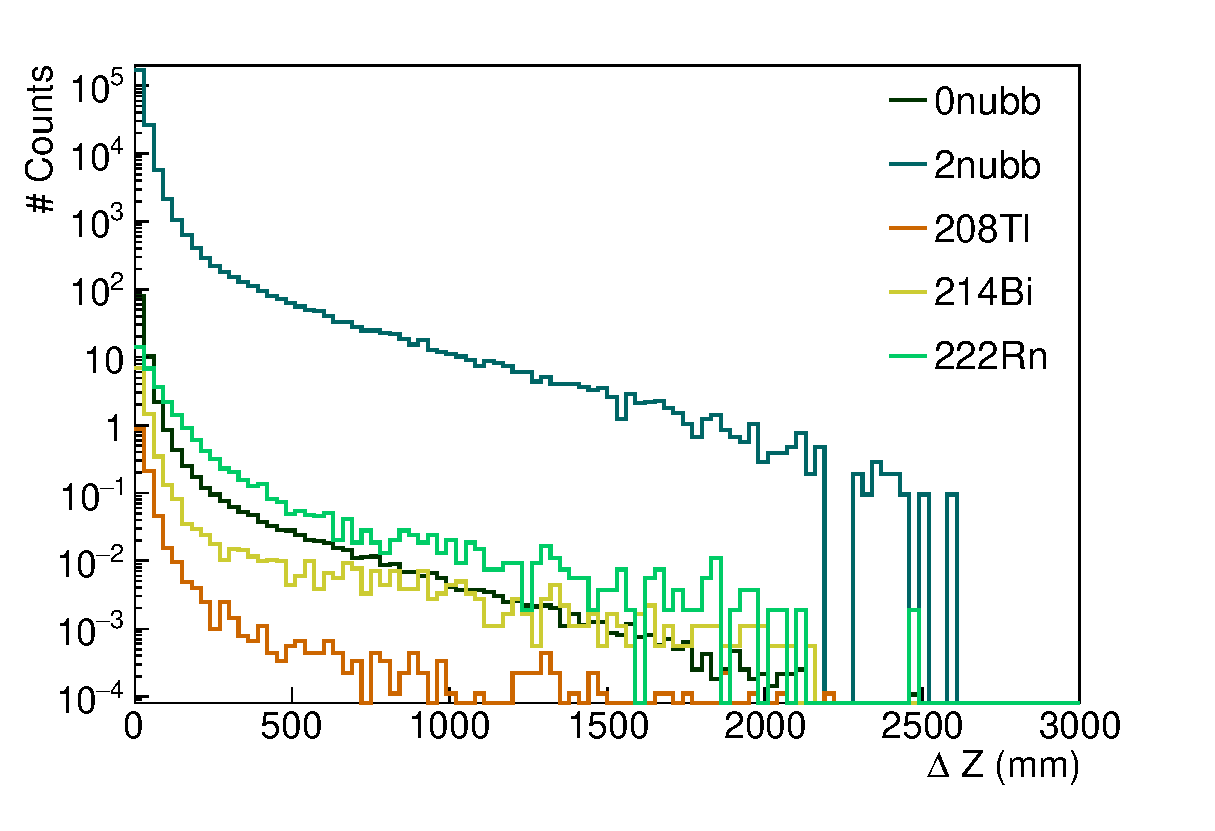
\includegraphics[width=0.8\textwidth]{Sensitivity/fig_sensitivity/Vertex_distance.eps}
  \caption{
    \label{fig:vertex_dist}}
\end{figure}
The two electrons of $\zeronu$ and $\twonu$ decays are actually emitted from the same vertex, unlike natural isotope disintegrations.
* a finir*

Fig.~\ref{fig:cont_vertex} displays the limit set on $\Tbeta$ as a function of the applied cut-off on the vertex distance in the Z direction.
\begin{figure}[h]
  \centering
  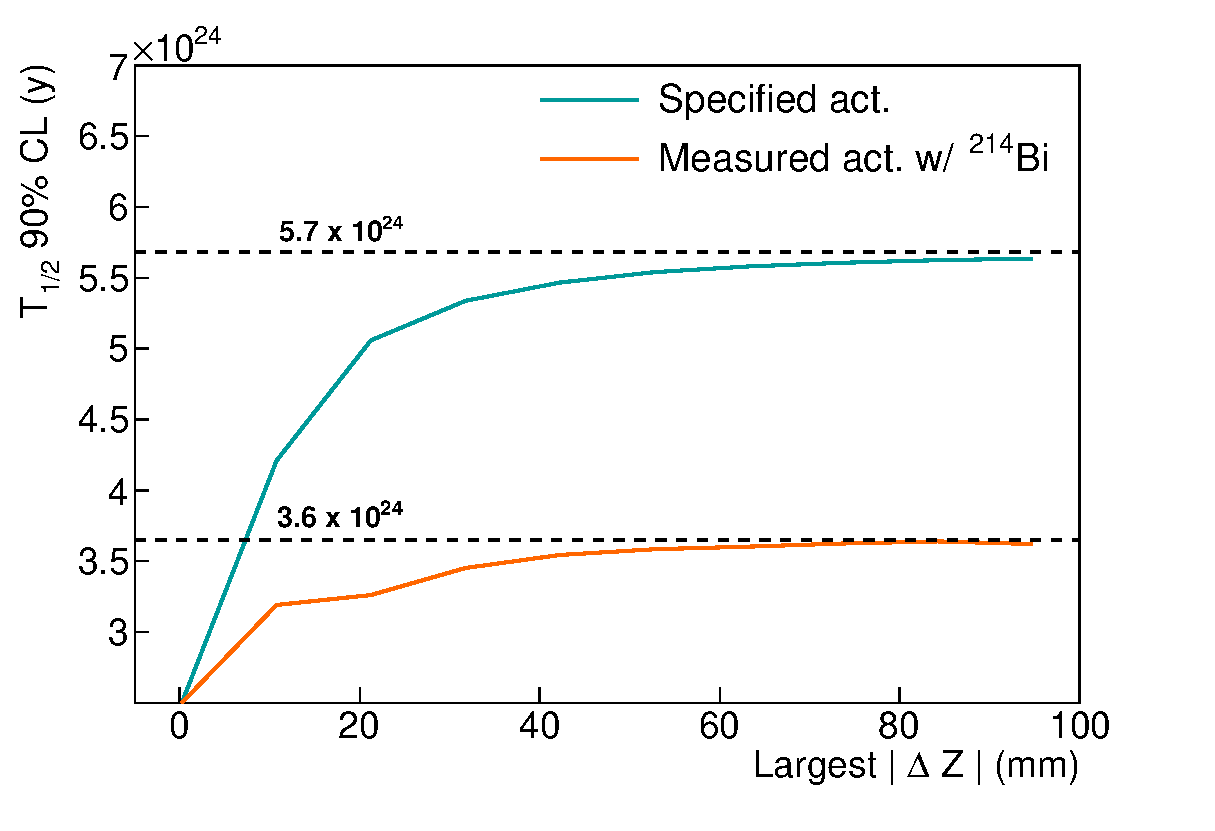
\includegraphics[width=0.8\textwidth]{Sensitivity/fig_sensitivity/contamination_vertex.eps}
  \caption{
    \label{fig:cont_vertex}}
\end{figure}
For all three contamination levels, we reach a plateau for a cut-off of more than 60 mm in $\Delta z$.
The same conclusions apply to the $\Delta y$ cut-off.
These results are consistent with the findings of the previous analysis conducted by Steven Calvez, asserting the two reconstructed vertices on source foils should not be separated by more than $60$ mm horizontally ($|\Delta y| < 60$ mm), and by more than $70$ mm vertically ($|\Delta z| < 70$ mm).


These cuts follow the NEMO-$3$ analysis on the background rejection, whose effectiveness were lately confirmed for the SuperNEMO demonstrator~\cite{docdb:calvez2014}.
first-order and topological cuts have efficiencies of selection differing for each type of decay.
We computed these efficiencies, presented in Tab.~\ref{tab:selections_eff}.
\begin{table}[h]
  \centering
  \begin{tabular}{|c|c|c|c|}
    \hline
    & first-order cuts (\%) & Internal probability (\%) & Vertex distance (\%)  \\
    \hline\hline
    $\zeronu$  & $26.9$ & $25.3$ & $24.2$ \\
    $\twonu$  & $9.16$ & $8.57$ & $8.01$ \\ %% (à recalculer avec 2nu2mev)
    \Tl  & $0.106$ & $0.0888$ & $0.0821$\\
    \Bi  & $0.168$ & $0.151$ & $0.140$ \\
    \Rn  & $0.0169$ & $7.3\times 10^{-5}$ & $4.27\times 10^{-5}$\\
    \hline
  \end{tabular}
  \caption{Number of selected $2e$ topologies compared with the total number of simulated decays, for first-order cuts and topological cuts.
  \label{tab:selections_eff}}
\end{table}
We observe topological cuts allow the selection of a high proportion of $\zeronu$ signal events, while rejecting most of the background events, especially the Radon-induced \Bi\ decays inside the tracker.
%% As explained in Sec.~\ref{sec:sensitivity_simus}, the \Bi\ decays following a Radon contamination of the tracker are not emitted from the source, but mainly from the tracker wires.
%% The internal probability and vertices separation can therefore help discriminate such events from signal events.

After looking at the effect of contaminations on the sensitivity, we review the influence of the magnetic field inside the detector.


\section{Impact of the magnetic field on the sensitivity}


The SuperNEMO demonstrator was originally designed with a copper coil, similarly to NEMO-$3$, delivering a magnetic field inside the tracker volume, aiming to provide an electron/positron discrimination.
This $25$~G magnetic field is high enough to bend the trajectory of the few MeV electrons and positrons of interest for SuperNEMO, without preventing them from reaching the calorimeter.
In practice, this magnetic field is mainly used to identify and reject the electron-positron pairs created by high energy $\gamma$’s, themselves emitted after a neutron capture.
In this study, however, we did not consider the contribution of external background in determining the best sensitivity.
We will therefore focus on evaluating the influence of the presence of the magnetic field on the rejection of internal and wire chamber backgrounds.
%% It is also very useful to better identify the crossing electron events, mostly coming from a 212 Bi contamination on the surface of the calorimeter, as explained in Section 3.2.4.
%% For instance, as shown in Figure 4.1, NEMO-3 observed three events in the [2.8;3.2]MeV region of interest in the one electron one positron channel and two events, induced by high energy $\gamma$’s from neutron capture, with energies higher than 4 MeV.


%% As described in Sec.~\ref{sec:magnetic_field}, the presence of a magnetic field of $25$ G could influence the optical modules performances.
%% In the simulated detector, such effects are not yet implemented, therefore can't be observed in the framework of this analysis.
%% However, possible degradation of the event reconstruction efficiency.



\subsection{Simulations of the magnetic field inside the demonstrator and reconstructed track fit}

In order to study the influence of the magnetic field on the Selenium-$82$ $\zeronu$ sensitivity, the simulations and reconstructions of decays described in Sec.~\ref{sec:sensitivity_simus} have been performed in three different conditions:
\begin{itemize}
\item simulations with a $25$ G \emph{uniform} magnetic field (following recommendations \cite{CalvezThesis}),
\item simulations where the magnetic field is turned off,
\item simulations with a $25$ G \emph{mapped} magnetic field, taking into account more realistic variations of the magnetic field inside the detector~\cite{docdb:map_magnetic_field2015}.
\end{itemize}
Each magnetic field condition has the same number of simulated events, as summed up in Tab.~\ref{tab:sensitivity_simulations}.
Depending on the case considered, the electrons will not have the same trajectory curvature.
In the first uniform on-field case, the best track fit is performed by helices.
In the second off-field case, the motion of an electron is in a straight line.
The fitting algorithm have thus be modified to match line trajectories.
Finally, the best tracking option (line or helix) for the third mapped on-field case will be discussed in the next section.

We oppose in Fig.~\ref{fig:real_target_act} the $\Tbeta$ results with and without this field inside the detector.
A third result is also presented, with the mapped field.

\subsection{Impact of the magnetic field on signal background selections}

Among the various event selection criteria considered in Sec.~\ref{sec:sensitivity_ev_selection}, the last one is of primary importance with regard to the influence of the magnetic field on the final sensitivity of the detector.
Indeed, when the magnetic field is switched on, the charged particles of few MeV (as electrons and positrons) have a curved trajectories.
A particle is then identified as an electron when the trajectory fitting results in a negative curvature.
When the magnetic field is switched off, the trajectory of the charged particles takes place in a straight line\footnote{When we say this, we do not take into account possible deviations in the trajectory of the particles, due in particular to multiple scattering in the tracker.}.
This last selection criterion is then no longer applied.
Consequently, the number of identified $2e$ topologies, selected by the first-order cuts, are increased, for the signal and background simulated events.
To illustrate this effect, we give in Fig.~\ref{fig:eff_0nu_w_wo_B} the selection efficiency $\epsilon_{0\nu}$ as a function of the $2e$ total energy, for the two cases of magnetic field presented above.
\begin{figure}[h]
  \centering
  \includegraphics[width=0.8\textwidth]{Sensitivity/fig_sensitivity/Nbkg_field.pdf}
  \caption{The $\zeronu$ selection efficiency as a function of the $2e$ total energy, for the on-field (blue) and the off-field (orange) cases.
    The two corresponding region of interests are also displayed by coloured stripes.
    Here no optimised topological cut-offs have been applied.
    \label{fig:eff_0nu_w_wo_B}}
\end{figure}
The two coloured stripes represent the corresponding region of interests, of [$2.7$;$3.15$]~MeV for the \emph{on-field} case, and [$2.75$;$3.2$]~MeV for the \emph{off-field} case.
These results are presented for the specified contamination levels, but remain valid in all cases.
We clearly notice that, for the total energy interval [$0$;$4$] MeV, the number of $\zeronu$ events selected is higher in the off-field case, which confirms what we were saying above.

The $\zeronu$ selection efficiency in the region of interest directly impacts the final sensitivity, following Eq.~\eqref{eq:tbeta_limit}.
Indeed, the upper limit set on $\Tbeta$ depends on $\epsilon_{0\nu}$ as well as on $N_{0\nu}^{\text{excl.}}$, the number of signal events excluded.
Nevertheless, for such levels of contaminations, due to the Feldman-Cousins statistics, the latter has no effect on sensitivity, and only the $\zeronu$ selection efficiency in the region of interest plays a role.
For the two field cases of interest, these efficiencies are $\epsilon_{0\nu}^{\text{on-field}}=0.15\%>\epsilon_{0\nu}^{\text{off-field}}=0.12\%$.
The selection efficiency for the on-field case is favoured by the lower bound of the ROI.
In fact, the further this lower bound is shifted towards lower energies, the greater the selection efficiency.
Besides, slight variations of the upper bound have almost no impact.
As expected, this results in a decrease in sensitivity for the off-field case, giving
\begin{equation}
\Tbeta > 4.80\times 10^{24}\,\text{y}\qquad (90\% \text{CL})\,.
\end{equation}

However, this decrease in sensitivity when the field is switched off can be compensated by applying the topological cut-offs described in subsection~\ref{subsec:opti_ev_selection}.
We optimised these selections for each contamination level case, and for both field and no field cases.
In Fig.~\ref{fig:sensitivity_B} are presented the best values for $\Tbeta$, using optimised topological cut-offs, both for on-field (see Tab.~\ref{tab:cut_Pint}) and off-field cases.
\begin{figure}[h]
  \centering
  \includegraphics[width=1.1\textwidth]{Sensitivity/fig_sensitivity/contamination_Se_w_woB.pdf}
  \caption{Best limit set on $\zeronu$ half-life (top pad), and the corresponding ROI (bottom pad), as a function of the contamination level considered, for both on-field and off-field cases.
    \label{fig:sensitivity_B}}
\end{figure}
The topological cuts allow to increase the final sensitivity.
The $\Tbeta$ value for off-field case, taking the specified activities, goes from $4.80\times 10^{24}\,\text{y}$ to $6.22\times 10^{24}\,\text{y}$, an improvement of $30\%$.
Because of the higher level of selected $2e$ topologies, higher sensitivities can be reached for the off-field case than for the on-field case, if using optimised topological cut-offs.
More generally, by using first-order cuts as well as topological cuts adapted to each case, we achieve higher sensitivities for the off-field case.
We note, however, that for high contamination levels (i.e. measured activities with and without bismuth), the difference in sensitivity for the two magnetic field cases tends to decrease.

\subsection{Influence of the magnetic field on optical modules and reconstruction efficiency}

Studies have been lead to evaluate its influence on the optical modules and on the event reconstruction~\cite{CalvezThesis}\cite{internal:magnetic_field}.

SuperNEMO PMTs are protected from the external magnetic field by an iron shield.
Unfortunately, the latter do not perfectly protect the PMTs, and a residual magnetic field is measured inside the shieldings, leading to charge losses and worsened energy resolution.
It was shown that applying a $25$ G magnetic field, and protect the PMTs with iron magnetic shields would be optimal, but not without consequences.
In fact, for the recommended value of $25$ G for the magnetic field, PMT charge losses would be close to $8\%$, and the PMT energy resolution would be increased of $\sim 3\%$.
Moreover, the PMTs shieldings could themselves severely impact the shape of the field lines, as well as its strength.
In fact, with a $25$ G magnetic field generated by the copper coil, the magnetic shields are responsible for the field strength decreasing, and barely $10$ G is expected near the source foils.
Moreover, the magnetic field strength decreases quickly as we get closer to the calorimeter walls.
The reconstruction efficiency could therefore be greatly impacted:
the magnetic field intensity varying from the source foils to the calorimeter wall, electrons trajectory curvatures are not constant, and the track is less well fitted.
This effect is higher as the electron energy decreases.

Despite the fact that magnetic shields were designed and installed to protect the PMTs, this field can have a great impact on the calorimeter detection efficiency, and thus could degrade the detector's sensitivity to the $\zeronu$ decay.
If the studies cited have evaluated the influence of the presence of the magnetic field on the reconstruction efficiency of $\zeronu$ events, it remains to be seen its consequences on the final demonstrator sensitivity.



\section{Searching for the Neodymium-$150~\zeronu$ decay}
\label{sec:Nd}

This study was conducted jointly with the PhD student Axel Pin, from CENBG~\cite{}.
Although we both worked on the whole of the analysis, I presented in detail, in the previous sections, the results regarding the influence of the magnetic field.
Meanwhile, Axel Pin will present in detail the possibility of changing the Selenium material by Neodymium sources~\cite{AxelThesis}.
The current section aims at summarise the feasibility study on Neodymium sources.

In the case SuperNEMO demonstrates the feasibility of a large-scale tracko-calo experiment, we would examine the possibility of different source isotopes, as done on NEMO-$3$.
The \Nd\ has a more favourable $\Qbb$ than \Se, with $\Qbb = 3.37$ MeV, .
However, its $\Ttwonu$ is lower, with $9.1\times 10^{18}$~years [ref].
For this study, we keep the \Se\ values for the contaminations, despite different purification efficiencies for the two isotopes.


\begin{itemize}
\item préciser que compte-tenu du Z important du 150Nd, même si la demi-vie de la 2nu est assez faible, cela ne gêne pas trop car les effets coulombiens font que la 2nu ne contribue pas trop à haute énergie.
\item distribution t1/2 avec différents échantillons de simus (17.5 kg.y)
\end{itemize}

\section{The final detector sensitivity}

The final goal of the SuperNEMO demonstrator is to demonstrate that the NEMO technology is scalable to reach high half-life sensitivity on the $\zeronu$ decay.
It was therefore mandatory to study the case of the final detector sensitivity, consisting in building $20$ modules similar to the SuperNEMO demonstrator, to reach unprecedented levels on effective neutrino masses.



\section{Conclusion}
\begin{itemize}
\item Etude plus générale avec bkg externe+lab (reprendre chiffres NEMO3) + neutrons (cf NEMO3)
\item Plot général récap tous résultats
\item delayed cells->improvement, cf NEMO 3
\item ouverture sur possibilité d'étudier l'influence de la résolution en temps des PMs sur l'eff des coupures (Pint)
\item cellules tracker dead-> refaire analyse
\item manque de stat pour le neodyme car ROI haute E
\item légères diff avec résultats axel car légères diff dans sélections d'ev car utilisation PID
\item tenir compte de la dégradation en énergie dans les simus du au B
\item optimisation topo cuts : multivariate analysis peut être envisagée pour aller plus loin
\end{itemize}
